\documentclass[11pt,a4paper]{article}

\usepackage[margin=2.4cm]{geometry}
\usepackage{amsmath}
\usepackage{amssymb}
\usepackage{booktabs}
\usepackage{graphicx}
\usepackage[table]{xcolor}
\usepackage{caption}
\usepackage[colorlinks=true,linkcolor=black,citecolor=black,urlcolor=blue]{hyperref}
\usepackage{siunitx}

\captionsetup{font=small,labelfont=bf}
\newcommand{\rocof}{\ensuremath{\mathrm{RoCoF}}}
\newcommand{\Rtwo}{\ensuremath{R^{2}}}

\title{\textbf{Predictors of frequency risk, and how easily they are
faked}\\[2pt]
\large a spectral-clustering attempt, a two-column physical model,
and three layers of validation that reverse the answer twice}
\author{}
\date{}

\begin{document}
\maketitle
\vspace{-2.2\baselineskip}

\section{What is being predicted, and how it is scored}

\emph{Risk} is one number per operating state: the \SI{500}{\milli\second}
\rocof{} summed over the five worst buses and averaged over the twenty
hazard scenarios (the \texttt{rocof\_top5} column; the vertical axis of the
right-hand pane of Figure~\ref{fig:four}). The ensemble is 240 balanced
configurations of a frozen 100-bus toy grid, 16 draws at each of 15 SNSP
levels from 30\% to 100\%.

Sections~3--6 hold out \emph{configurations}: sixty configurations
(25\%, stratified by SNSP level) were held out before any modelling and read
once, at the end. Everything else --- the number of clusters, the feature
set, the ridge penalty --- was chosen by $20\times5$-fold cross-validation
inside the remaining 180. All models are fitted to $\log_{10}$ risk, so a
residual is a multiplicative error; the ``98\% band'' is the multiplicative
width of the central 98\% of residuals, and ``outliers'' counts held-out
configurations missed by more than 10\%.

\textbf{That protocol is not sufficient, and Section~8 shows why.} Every fold
of it shares the same twenty disturbances, so it cannot detect a feature that
has been built from those disturbances. The reader who wants the honest
numbers should read Section~8 before believing Table~\ref{tab:main}.

\section{The construction that was proposed}

The grid was cut into electrically coherent regions by spectral clustering
of the coupling matrix $K_{ij}$ --- the synchronising coefficients, i.e.\ the
network as the swing equations see it. With $L = I - D^{-1/2} K D^{-1/2}$,
the eigengap heuristic chooses $k$ maximising $\lambda_{k+1}-\lambda_k$; the
$k$ lowest eigenvectors are row-normalised and $k$-means clustered
(Ng--Jordan--Weiss). The partition depends only on the network, which never
varies, so it is computed once and every configuration is described by the
same regions.

This gives $k=4$ --- a clean north-west / north-east / south-east / south-west
cut, wind-heavy west against demand-heavy east, cutting 11\% of the total
coupling. \textbf{But it wins by a hair}: the gap at $k=4$ exceeds the
runner-up ($k=12$) by a factor of 1.01. A $10\times10$ mesh is not a
barbell, and that margin is the first warning.

Each configuration then gets, per region, its non-synchronous share, stored
energy $\sum H_i S_i$, primary reserve, mean distance to the nearest spinning
machine, and the ratio (non-synchronous output)$/\sum H_i S_i$. A continuous
alternative was also built: projections of the dispatch onto the ten slowest
Laplacian modes (\texttt{modal}), which is what a Fiedler vector actually is
before it is thresholded into a partition.

\section{Results}

\begin{table}[h]
\centering
\small
\caption{Held-out performance on the 60 configurations never used for
fitting or selection. $p$ is the number of columns.}
\begin{tabular}{lrrrrr}
\toprule
feature set & $p$ & test \Rtwo & 98\% band & worst miss & outliers \\
\midrule
SNSP alone                                    & 1  & 0.794 & 1.78$\times$ & 1.49$\times$ & 28/60 \\
SNSP, quadratic                               & 2  & 0.833 & 1.75$\times$ & 1.47$\times$ & 23/60 \\
\midrule
\rowcolor{gray!12}
$\log(\Pi/H)$, coefficients forced $(+1,-1)$  & 1  & 0.944 & 1.31$\times$ & 1.16$\times$ & 15/60 \\
\rowcolor{gray!12}
\textbf{swing}: $\log \Pi$, $\log H$ free     & 2  & \textbf{0.971} & 1.22$\times$ & 1.12$\times$ & \textbf{2/60} \\
\rowcolor{gray!12}
\ \ + reserve, distance to a machine          & 4  & \textbf{0.978} & 1.18$\times$ & 1.10$\times$ & \textbf{2/60} \\
\midrule
all system-wide columns                       & 12 & 0.928 & 1.39$\times$ & 1.22$\times$ & 19/60 \\
SNSP per region                               & 4  & 0.808 & 1.82$\times$ & 1.48$\times$ & 28/60 \\
all per-region features                       & 20 & 0.957 & 1.33$\times$ & 1.18$\times$ & 11/60 \\
projection onto 10 slowest modes              & 31 & 0.971 & 1.25$\times$ & 1.13$\times$ & 5/60 \\
\bottomrule
\end{tabular}
\label{tab:main}
\end{table}

The goal was met: against SNSP the trend narrows from 1.78$\times$ to
1.18$\times$ and outliers fall from 28 to 2 of 60. But the winner is not the
cluster model. It is a \textbf{two-column} model containing no geography at
all.

\section{Three controls say the clustering is not doing the work}

\begin{enumerate}\itemsep2pt
\item \textbf{Partition control.} The identical 20-column construction on
partitions that are not spectral: spectral 0.957, a naive geographic
quartering drawn with a ruler 0.956, random partitions of identical sizes
0.953 on average. The spectral cut beats only \textbf{12 of 20} random
partitions.

\item \textbf{Basis control.} The \texttt{modal} family on the ten
\emph{slowest} modes scores 0.971; on the ten \emph{fastest} modes, 0.970.
The fast modes are single-bus wiggles with no regional meaning whatever. If
they predict as well as the Fiedler vector, the spectrum is not what is being
used --- the dimension is. Random orthonormal rotations reach 0.963.

\item \textbf{$k$ sweep.} Held-out \Rtwo{} for the cluster families is flat
and non-monotonic from $k=2$ to $k=12$ (0.86 to 0.95), consistent with an
eigengap that had no strong preference to begin with.
\end{enumerate}

\section{Why there was nothing local to find}

The diagnostic that explains all three controls: evaluate the same
\SI{500}{\milli\second} window on the centre-of-inertia frequency --- the
whole grid as a single machine. That one system-wide number already accounts
for $\Rtwo = 0.953$ of $\log$ risk. The five worst buses run
$7.94\times$ (s.d.\ 0.83) the system-wide reading, and only \textbf{11.8\%}
of the target's variance is local amplification. The score is a system-wide
quantity wearing a local costume, so a partition has almost nothing to
resolve.

\paragraph{Does this hold for \texttt{rocof\_top1}?} Yes, but less strongly,
and the trend is exactly as expected. Narrowing from five worst buses to the
single worst bus raises the local share, because averaging over five buses
averages local variation away:

\begin{table}[h]
\centering
\small
\begin{tabular}{lrrr}
\toprule
target & \Rtwo{} vs.\ system-wide & local share of variance & spectral beats \\
\midrule
\texttt{rocof\_top1}  & 0.938 & 19.1\% & 15 of 20 random \\
\texttt{rocof\_top5}  & 0.953 & 11.8\% & 12 of 20 random \\
\texttt{rocof\_top10} & 0.960 & \ \ 8.8\% & --- \\
\bottomrule
\end{tabular}
\end{table}

So \texttt{rocof\_top1} is genuinely more local, and the spectral partition
does correspondingly better --- 15 of 20 rather than 12 of 20. That is the
right direction, and it is still not a result: the target remains 94\%
system-wide, the spectral cut still only ties the ruler-drawn quartering
($+0.002$), and slow and fast modes still tie exactly (0.962 versus 0.962).
The conclusion survives the sharper target. Incidentally the deviation
scores are \emph{more} system-wide still (\texttt{dev\_top5}: $\Rtwo=0.997$,
4.8\% local), which makes sense --- a nadir develops over seconds, by which
time the grid has synchronised, whereas a \SI{500}{\milli\second} \rocof{}
is read while it has not.

\section{So why \emph{do} these predictors beat SNSP?}

This is the substantive point, and it has nothing to do with geography.

\paragraph{What the hazard variable is.} First, a definition, because the
symbol is easy to misread. Every configuration in this ensemble is
\emph{balanced} before anything happens: $\sum_i P_i = 4\times10^{-16}$ p.u.
There is no standing power difference and none is being regressed on. The
regressor is the aggregate \emph{size of the contingency set},
\begin{equation}
\Pi \;\equiv\; \sum_{k=1}^{E}\bigl|\Delta P_k\bigr|,
\qquad
\Delta P_k \;=\; \textstyle\sum_i U_{ik},
\label{eq:hazard}
\end{equation}
where $U_{\cdot k}$ is the injection step that disturbance $k$ applies and
$E=20$. So $\Delta P_k$ is the imbalance each contingency \emph{creates} at
the instant it occurs --- a \SI{0.4}{p.u.} demand block switching in, a wind
farm losing its output --- not any imbalance present beforehand. $\Pi$ varies
between configurations because the disturbance set is \emph{sourced}: each
event scales with its own source, so a wind farm running harder has more to
lose when it trips. It is known from the dispatch before any solve.

\paragraph{Why those two variables.} For a single event the swing equation
for the centre of inertia gives
\begin{equation}
\frac{\mathrm{d}f}{\mathrm{d}t}\Big|_{t=0} \;=\; \frac{f_0\,\Delta P_k}{2\sum_i H_i S_i},
\label{eq:swing}
\end{equation}
and since the target averages over events and the response is linear in the
step, the aggregate $\Pi$ and the stored energy $\sum_i H_iS_i$ are the two
quantities the physics says should matter. Risk is a \emph{ratio of two
extensive quantities}: megawatts that can be lost, over stored energy to
absorb them. SNSP is neither. It is
\begin{equation}
\mathrm{SNSP} \;=\; \frac{P_{\text{non-sync}}}{P_{\text{total}}},
\end{equation}
a dimensionless \emph{share}. Three consequences follow, and together they
are the entire gap in Table~\ref{tab:main}.

\paragraph{(i) It is a proxy for the denominator, and an imperfect one.}
Across the ensemble SNSP correlates with $\log\sum H_i S_i$ at $r=-0.919$.
That is why SNSP works at all: displacing synchronous generation removes
inertia. But it is a correlation, not an identity, because \emph{which}
machines are displaced is free. At a fixed SNSP level the stored energy
still ranges by 28\% of its mean (median across levels; up to 51\%). Used
alone, $\log(1/H)$ already scores 0.842 against SNSP's 0.794 --- the proxy is
worse than the thing it proxies for.

\paragraph{(ii) It is nearly blind to the numerator.} SNSP correlates with
$\log \Pi$ at only $r=+0.336$. The size of the largest credible loss
depends on what is actually running and how hard --- a loaded HVDC link, a
radial wind farm at full output --- and a \emph{share} cannot see it. At
fixed SNSP the hazard still ranges by 23\% of its mean. This is the piece
SNSP misses most completely, and it is why adding $\log \Pi$ to $\log H$
moves outliers from 15 to 2.

\paragraph{(iii) A ratio discards the scale.} Two configurations with the
same SNSP at different demand carry the same label and different physics. In
this ensemble demand is fixed, which flatters SNSP considerably; on a real
system, where demand varies by a factor of two between night and peak, the
defect would be far worse.

\paragraph{The fitted exponents are not $(+1,-1)$, and that is itself
physics.} Forcing the coefficients to the purely inertial values --- fitting
only an offset to $\log\Pi - \log\sum H_iS_i$ --- already reaches
$\Rtwo=0.944$. Freeing them reaches $0.971$, at
\begin{equation}
\log_{10}\rocof \;=\; +1.285\,\log_{10}\Pi \;-\; 0.645\,\log_{10}\textstyle\sum_i H_iS_i
\;+\; \text{const}.
\end{equation}
The departure is not noise. The score is measured over a
\SI{500}{\milli\second} window, not at $t=0$: by then load damping and
governor action have begun to arrest the frequency, and in the settled limit
the offset is $\Delta P/(R+D)$, independent of inertia altogether. The
inertia exponent therefore interpolates between $-1$ (instantaneous) and $0$
(settled), and $-0.645$ is where \SI{500}{\milli\second} falls for this
system. Consistently, the residual of the forced model correlates at
$r=+0.879$ with stored energy and $r=+0.879$ with reserve --- the pure
inertial form over-weights inertia. The hazard exponent exceeds $1$ because
$\Pi$ sums twenty events with different spatial signatures, so risk is
proportional to a \emph{weighted} sum of the $|\Delta P_k|$ rather than to
their plain total, and the two regressors are mildly correlated
($r=-0.235$). Equation~\ref{eq:swing} is thus the right \emph{motivation}
for the two variables, not a law being confirmed to two decimal places.

\paragraph{What the elaborate feature sets were actually doing.} Every
per-region and modal feature is a \emph{linear functional of the per-bus
dispatch and inertia vectors}. Summing $H_iS_i$ over region $j$, or
projecting it onto eigenvector $v_m$, both produce weighted sums of the same
100 numbers. Given twenty or thirty such functionals, a linear model can
reconstruct the two aggregates in Equation~\ref{eq:swing} to good accuracy
--- and \emph{any} spanning set of functionals will do, which is precisely
what the partition and basis controls found. The eigenvectors are one basis
among many; the fast modes are another; a random rotation is a third. They
all work because they all span the same thing. Supporting this directly: the
raw per-unit state (18 unit outputs plus 5 inertias plus 5 droops, no
partition and no spectrum) scores 0.943, in the same band.

The clustering, in other words, was an expensive and indirect way of
recovering $\Pi$ and $\sum_i H_iS_i$. Computing them straight from the dispatch is
two columns, needs no eigenvector, and does better.

\begin{figure}[t]
\centering
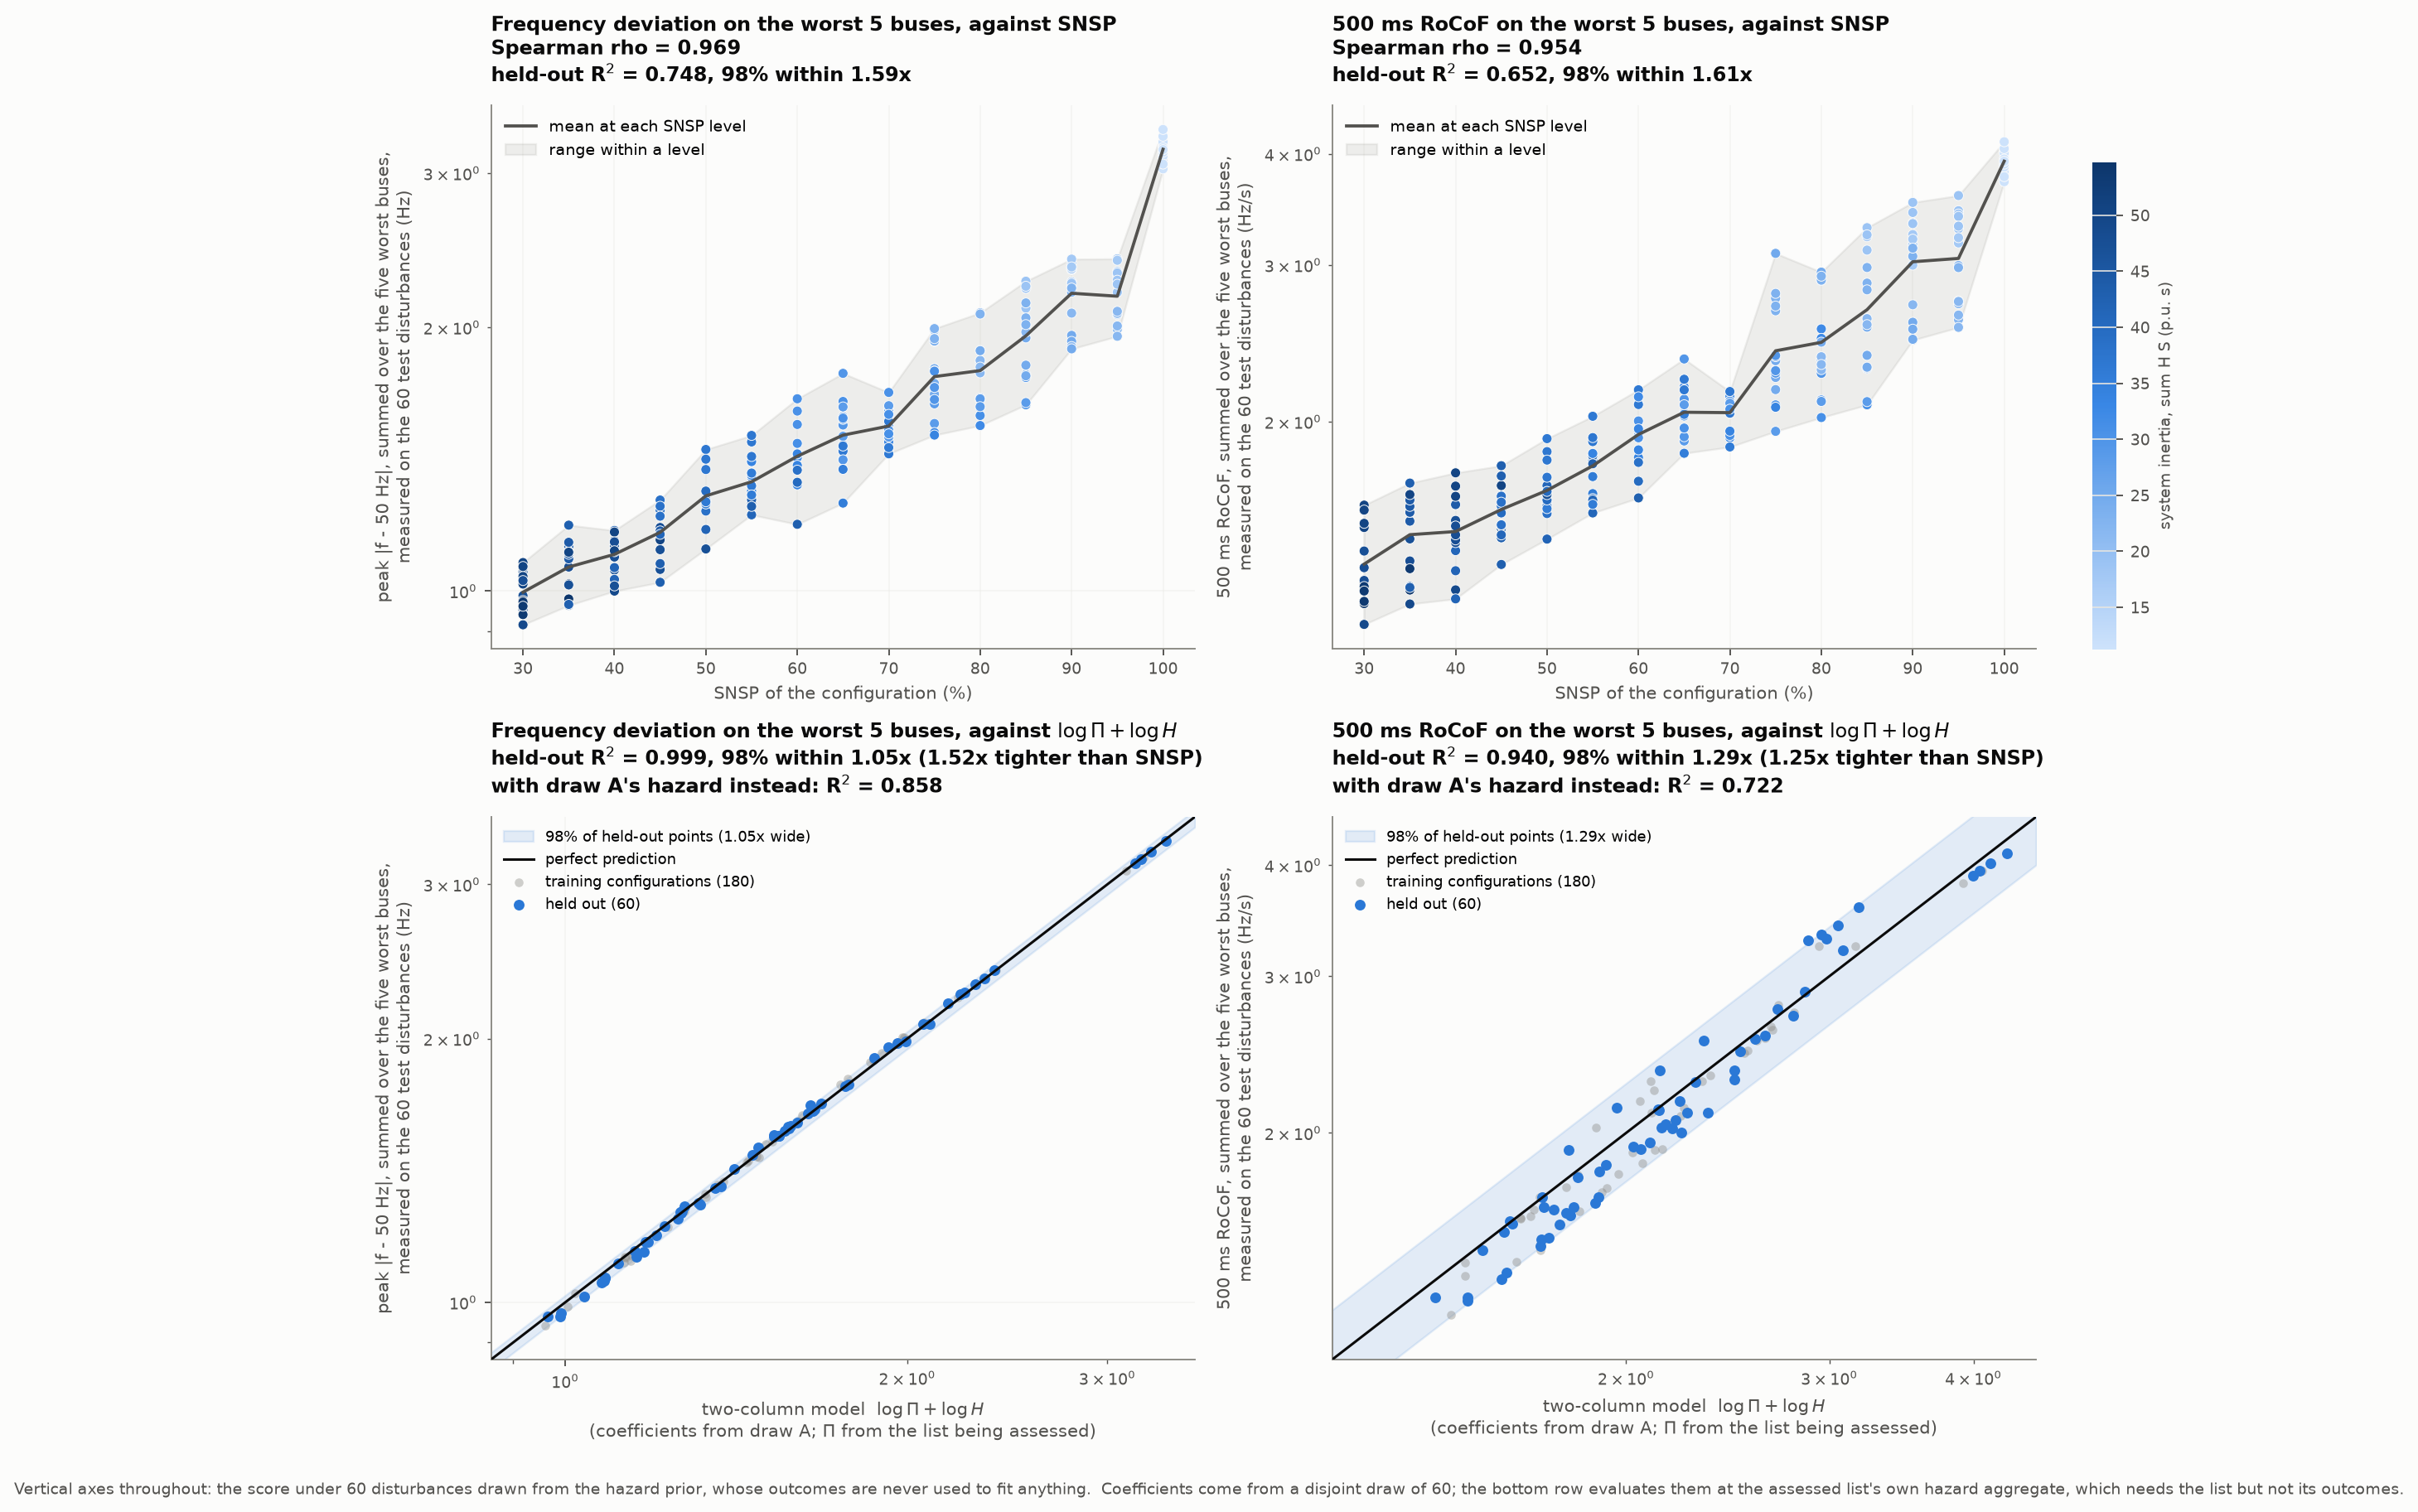
\includegraphics[width=\textwidth]{../figures/fig11_topbus_vs_predictor.png}
\caption{Vertical axes throughout: the score under draw~B, sixty
disturbances sampled from the hazard prior whose outcomes are never used to
fit anything. Top: against SNSP. Bottom: against $\log\Pi + \log H$, two
coefficients fitted on the disjoint draw~A and evaluated at the assessed
list's own hazard aggregate. The 98\% band narrows 1.52$\times$ for the
deviation and 1.25$\times$ for the \rocof{}; each title also quotes what the
same model scores holding a stale list.}
\label{fig:four}
\end{figure}

\section{Three layers of validation}

Everything above holds out configurations. It never holds out
\emph{disturbances} --- and $\Pi$ is summed over exactly the twenty
disturbances whose outcomes define the target. The predictor knows the
realised sizes of the very events it is scored on, and no amount of holding
out configurations can see that. What follows is what happened when the
protocol was tightened twice.

\subsection*{Layer 1: hold out configurations (Sections 3--6)}
Sixty configurations held out, one fixed twenty-event set throughout.
The two-column swing model reaches $\Rtwo = 0.978$ with 2 outliers of 60 and
looks decisive. It is not trustworthy, for the reason just given.

\subsection*{Layer 2: split the frozen event set in half --- and why this
was also wrong}
Fit on ten of the twenty disturbances, rank configurations on the disjoint
ten. Under this test the swing model collapsed to $\rho = 0.698$, the worst
of everything tried, below plain SNSP by $0.124$
($p = 3\times10^{-13}$, 36 of 40 splits). Taken at face value that says
$\Pi$ is pure leakage.

\textbf{It is not, and the test was faulty.} The twenty events are a
\emph{designed} set with a fixed composition --- five demand steps, eight wind
drops, four unit trips. A random half of them is not a representative sample
of anything: the two halves carry different mixtures, so $\Pi_A$ and $\Pi_B$
measure different quantities. Their aggregates \emph{anti}-correlate,
$\mathrm{corr}(\log\Pi_A,\log\Pi_B) = -0.385 \pm 0.109$ over 200 splits, and
the collapse follows from that artefact rather than from any property of the
hazard.

\subsection*{Layer 3: sample two representative draws from a hazard prior}
The correct version of the same question. Define a prior over disturbances of
the same six families with the location and severity \emph{drawn} rather than
chosen --- a demand block of \SIrange{0.2}{0.6}{p.u.} at any city, a front
taking \SIrange{30}{90}{\percent} of any farm's output, a trip of any unit
capped at one machine. Draw two independent stratified samples of sixty.
Both are representative of the same distribution; they contain different
disturbances. Fit on draw~A, predict the score under draw~B.

The diagnostic reverses immediately:
$\mathrm{corr}(\log\Pi_A,\log\Pi_B) = +0.650$, and $\log\Pi_A$ correlates at
$+0.899$ with the closed-form $\mathbb{E}|\Delta P|$ under the prior. $\Pi$
\emph{is} a property of the operating state --- the expected megawatts at risk
given the dispatch --- estimated with sampling noise. With ten events from a
designed set that noise swamped it; with sixty drawn events it does not.

\begin{table}[h]
\centering
\small
\caption{Fit on draw~A, predict the score under the independent draw~B.
Sixty held-out configurations; bootstrap 90\% intervals over them.}
\begin{tabular}{lrrr}
\toprule
model & columns & test \Rtwo & 90\% CI \\
\midrule
\emph{ceiling: the measured score on draw A} & --- & \emph{0.792} & [0.706, 0.843] \\
\midrule
projection onto 10 slowest modes & 31 & 0.769 & [0.676, 0.824] \\
all per-region features          & 20 & 0.765 & [0.665, 0.826] \\
\rowcolor{gray!12}
$\log\Pi + \log H$               & \textbf{2} & \textbf{0.722} & [0.595, 0.795] \\
every system-wide column         & 12 & 0.716 & [0.575, 0.798] \\
inertia only                     & 1  & 0.686 & [0.573, 0.752] \\
SNSP alone                       & 1  & 0.652 & [0.432, 0.776] \\
\bottomrule
\end{tabular}
\label{tab:draw}
\end{table}

The swing model does not collapse. It reaches 91\% of the ceiling and beats
SNSP by $+0.077$ in \Rtwo{}. On rank correlation the ordering differs
slightly --- per-region features $0.970$, modal $0.962$, SNSP $0.943$, swing
$0.932$, against a ceiling of $0.964$ --- so the two-column model recovers the
level better than the ordering.

\paragraph{But nothing here is resolvable.} Every paired bootstrap interval
straddles zero: swing $-$ SNSP $= +0.077$ $[-0.009,+0.186]$; swing $-$ inertia
alone $= +0.034$ $[-0.022,+0.088]$; per-region $-$ swing $= +0.046$
$[-0.005,+0.105]$. With sixty test configurations that is the resolution
available. The defensible statement is that the swing model, the spatial
families and SNSP all sit in one band, with swing and the spatial families
probably ahead of SNSP.

\subsection*{Layer 3b: two questions, not one}
Table~\ref{tab:draw} answers the harder of two distinct questions, and it is
worth separating them because the model is far better at one than the other.

\begin{description}\itemsep2pt
\item[(a) \emph{Under our hazard prior, what is the expected risk?}] Here the
contingency list of the future is unknown, and the best available hazard
column is $\mathbb{E}|\Delta P|$ under the prior --- or a stale estimate of it
from an old list. This is Table~\ref{tab:draw}: $\Rtwo = 0.722$ for the RoCoF,
$0.858$ for the deviation.
\item[(b) \emph{Given \emph{this} contingency list, how risky is this
configuration?}] Here the list is known. And $\Pi$ for a list is a sum of
injection steps --- computable from the dispatch and the list alone, with no
solve. Knowing which disturbances you will be assessed against is not knowing
what they will do; an operator has the list before running any study.
\end{description}

Evaluating the \emph{same} coefficients, fitted on draw~A, at draw~B's own
hazard aggregate answers (b):

\begin{table}[h]
\centering
\small
\caption{Coefficients fitted on draw~A throughout; the score is always
draw~B's, whose outcomes are never used. The last column plugs draw~B's own
$\Pi$ into the fitted map --- the list, not its results.}
\begin{tabular}{lrrr}
\toprule
score & SNSP & $\log\Pi_A + \log H$ & $\log\Pi_B + \log H$ \\
      & (cannot adapt) & (stale list) & (assessed list) \\
\midrule
500 ms RoCoF, worst 5 & 0.652 & 0.722 & \textbf{0.940} \\
deviation, worst 5    & 0.748 & 0.858 & \textbf{0.999} \\
\bottomrule
\end{tabular}
\label{tab:applied}
\end{table}

Two things follow. First, most of the gap in Table~\ref{tab:draw} was not the
model failing but a \emph{level} offset: draw~B's sampled disturbances happen
to be \SI{9.5}{\percent} milder than draw~A's, so a predictor holding the old
list over-predicts by a constant. SNSP has no mechanism to notice this;
$\log\Pi + \log H$ corrects for it exactly, because the hazard aggregate of
the new list is a quantity you can compute. That adaptability is a property
SNSP structurally cannot have.

Second, $\Rtwo = 0.999$ on the deviation should be read with care. It is not
suspicious, it is the linear response showing through: the deviation is
\SI{99.7}{\percent} a system-wide quantity (Section~5), and the settled
system-wide offset is $\Delta P/(R+D)$, so the score is very nearly
$\Pi$ divided by a damping term that this ensemble's inertia column tracks
closely ($r = 0.74$ between $\log$ reserve and $\log$ inertia). The two-column
model is recovering an analytic solution. On a real system, with protection,
saturation and genuine nonlinearity, it would not be this clean --- the number
is a property of the toy model as much as of the predictor.

\paragraph{Which argues for the two-column model.} If the families cannot be
separated on accuracy, they can be separated on how much freedom they have to
be wrong. $\log\Pi + \log H$ carries two fitted coefficients; the per-region
set carries twenty and the modal set thirty-one, on 180 training rows. It
also states its own assumption openly: it needs a hazard \emph{model} to
compute $\Pi$, which is exactly the contingency list an operator already
maintains --- and Layer 3 shows that the specific realisation of that list does
not matter, only the distribution it is drawn from.

\section{Conclusions}

\begin{enumerate}\itemsep2pt
\item \textbf{The validation protocol, not the model, decided the answer ---
twice.} Holding out configurations alone made a leaky model look decisive;
halving a designed event set made the same model look worthless. Only a
hazard prior with two representative draws measures what was actually wanted.
\item \textbf{$\Pi$ is a legitimate state variable.} Two independent
sixty-event draws agree on it at $r=+0.650$ and it tracks the closed-form
$\mathbb{E}|\Delta P|$ at $+0.899$. It is the expected megawatts at risk given
the dispatch, not a memorised property of one contingency list.
\item \textbf{On a fresh draw, $\log\Pi + \log H$ predicts well}: $\Rtwo =
0.722$ against a ceiling of $0.792$, ahead of SNSP's $0.652$, with two fitted
coefficients. Its earlier collapse was an artefact of Layer 2; its earlier
brilliance was an artefact of Layer 1.
\item \textbf{Told which contingency list it is being assessed against ---
which needs the list, not its outcomes --- it reaches $\Rtwo = 0.940$ on the
RoCoF and $0.999$ on the deviation}, against SNSP's $0.652$ and $0.748$. The
hazard aggregate of a new list is computable without a solve, so the model
adapts to a change of list; SNSP structurally cannot. This is the strongest
honest claim available, and Figure~\ref{fig:four} is drawn on it.
\item \textbf{No family is separable from another here.} All the bootstrap
intervals overlap. Parsimony is then the tie-breaker, and it favours the
two-column model over twenty or thirty spatial columns.
\item The spectral clustering remains untested rather than refuted, for the
reason in Section~5: at 88--95\% system-wide content there is too little local
variance for a spatial feature to resolve. It is nominally top of
Table~\ref{tab:draw}, but not separably so.
\end{enumerate}

\paragraph{Caveats.} With 60 held-out configurations, differences below
about $0.02$ in \Rtwo{} are not resolvable, and several comparisons above
sit inside that. The \texttt{modal} family fits 31 columns on 180 training
rows, a thin ratio even under ridge. Demand is constant across this
ensemble, which flatters SNSP. The toy grid offers only about
twenty-four possible disturbance locations (thirteen farms, five cities, six
infeeds), so two sixty-event draws share twenty-one of them and differ mainly
in severity and multiplicity rather than in place; a genuinely independent
contingency list on a larger network would be a stronger test. Layer 3 also
assumes the prior is correct --- it tests generalisation across draws, not
against a misspecified hazard model, which
\texttt{risk\_predictor.cross\_hazard\_model} probes separately and where the
hazard term does lose to inertia alone.

\end{document}
